\documentclass{anstrans}
%%%%%%%%%%%%%%%%%%%%%%%%%%%%%%%%%%%
\title{Hydrogen Economy in Champaign-Urbana, IL}
\author{Roberto E. Fairhurst Agosta, Samuel G. Dotson, Kathryn D. Huff}

\institute{
University of Illinois at Urbana-Champaign, Dept. of Nuclear, Plasma, and Radiological Engineering\\
ref3@illinois.edu
}

%%%% packages and definitions (optional)
\usepackage{graphicx} % allows inclusion of graphics
\usepackage{booktabs} % nice rules (thick lines) for tables
\usepackage{microtype} % improves typography for PDF
\usepackage{xspace}
\usepackage{tabularx}
\usepackage{floatrow}
\usepackage{subcaption}
\usepackage{enumitem}
\usepackage{placeins}
\usepackage{amsmath}
\usepackage[acronym,toc]{glossaries}
\newacronym[longplural={metric tons of heavy metal}]{MTHM}{MTHM}{metric ton of heavy metal}
\newacronym{ABM}{ABM}{agent-based modeling}
\newacronym{ACDIS}{ACDIS}{Program in Arms Control \& Domestic and International Security}
\newacronym{AHTR}{AHTR}{Advanced High Temperature Reactor}
\newacronym{ANDRA}{ANDRA}{Agence Nationale pour la gestion des D\'echets RAdioactifs, the French National Agency for Radioactive Waste Management}
\newacronym{APP}{APP}{Abbott Power Plant}
\newacronym{ANL}{ANL}{Argonne National Laboratory}
\newacronym{API}{API}{application programming interface}
\newacronym{ARCH}{ARCH}{autoregressive conditional heteroskedastic}
\newacronym{ARE}{ARE}{Aircraft Reactor Experiment}
\newacronym{ARFC}{ARFC}{Advanced Reactors and Fuel Cycles}
\newacronym{ARMA}{ARMA}{autoregressive moving average}
\newacronym{ASME}{ASME}{American Society of Mechanical Engineers}
\newacronym{ATWS}{ATWS}{Anticipated Transient Without Scram}
\newacronym{BDBE}{BDBE}{Beyond Design Basis Event}
\newacronym{BIDS}{BIDS}{Berkeley Institute for Data Science}
\newacronym{BOL}{BOL}{Beginning-of-Life}
\newacronym{BSD}{BSD}{Berkeley Software Distribution}
\newacronym{CAFCA}{CAFCA}{ Code for Advanced Fuel Cycles Assessment }
\newacronym{CASL}{CASL}{Consortium for Advanced Simulation of Light Water Reactors}
\newacronym{CDTN}{CDTN}{Centro de Desenvolvimento da Tecnologia Nuclear}
\newacronym{CEA}{CEA}{Commissariat \`a l'\'Energie Atomique et aux \'Energies Alternatives}
\newacronym{CI}{CI}{continuous integration}
\newacronym{CNEC}{CNEC}{Consortium for Nonproliferation Enabling Capabilities}
\newacronym{CNEN}{CNEN}{Comiss\~{a}o Nacional de Energia Nuclear}
\newacronym{CNERG}{CNERG}{Computational Nuclear Engineering Research Group}
\newacronym{COSI}{COSI}{Commelini-Sicard}
\newacronym{COTS}{COTS}{commercial, off-the-shelf}
\newacronym{CSNF}{CSNF}{commercial spent nuclear fuel}
\newacronym{CTAH}{CTAHs}{Coiled Tube Air Heaters}
\newacronym{CUBIT}{CUBIT}{CUBIT Geometry and Mesh Generation Toolkit}
\newacronym{CURIE}{CURIE}{Centralized Used Fuel Resource for Information Exchange}
\newacronym{DAG}{DAG}{directed acyclic graph}
\newacronym{DANESS}{DANESS}{Dynamic Analysis of Nuclear Energy System Strategies}
\newacronym{DBE}{DBE}{Design Basis Event}
\newacronym{DESAE}{DESAE}{Dynamic Analysis of Nuclear Energy Systems Strategies}
\newacronym{DHS}{DHS}{Department of Homeland Security}
\newacronym{DOE}{DOE}{Department of Energy}
\newacronym{DRACS}{DRACS}{Direct Reactor Auxiliary Cooling System}
\newacronym{DRE}{DRE}{dynamic resource exchange}
\newacronym{DSNF}{DSNF}{DOE spent nuclear fuel}
\newacronym{DYMOND}{DYMOND}{Dynamic Model of Nuclear Development }
\newacronym{EBS}{EBS}{Engineered Barrier System}
\newacronym{EDZ}{EDZ}{Excavation Disturbed Zone}
\newacronym{EIA}{EIA}{U.S. Energy Information Administration}
\newacronym{EPA}{EPA}{Environmental Protection Agency}
\newacronym{EP}{EP}{Engineering Physics}
\newacronym{FCO}{FCO}{Fuel Cycle Options}
\newacronym{FCT}{FCT}{Fuel Cycle Technology}
\newacronym{FCWMD}{FCWMD}{Fuel Cycle and Waste Management Division}
\newacronym{FEHM}{FEHM}{Finite Element Heat and Mass Transfer}
\newacronym{FEPs}{FEPs}{Features, Events, and Processes}
\newacronym{FHR}{FHR}{Fluoride-Salt-Cooled High-Temperature Reactor}
\newacronym{FLiBe}{FLiBe}{Fluoride-Lithium-Beryllium}
\newacronym{GCAM}{GCAM}{Global Change Assessment Model}
\newacronym{GDSE}{GDSE}{Generic Disposal System Environment}
\newacronym{GDSM}{GDSM}{Generic Disposal System Model}
\newacronym{GENIUSv1}{GENIUSv1}{Global Evaluation of Nuclear Infrastructure Utilization Scenarios, Version 1}
\newacronym{GENIUSv2}{GENIUSv2}{Global Evaluation of Nuclear Infrastructure Utilization Scenarios, Version 2}
\newacronym{GENIUS}{GENIUS}{Global Evaluation of Nuclear Infrastructure Utilization Scenarios}
\newacronym{GPAM}{GPAM}{Generic Performance Assessment Model}
\newacronym{GRSAC}{GRSAC}{Graphite Reactor Severe Accident Code}
\newacronym{GUI}{GUI}{graphical user interface}
\newacronym{HLW}{HLW}{high level waste}
\newacronym{HPC}{HPC}{high-performance computing}
\newacronym{HTC}{HTC}{high-throughput computing}
\newacronym{HTGR}{HTGR}{High Temperature Gas-Cooled Reactor}
\newacronym{IAEA}{IAEA}{International Atomic Energy Agency}
\newacronym{IEMA}{IEMA}{Illinois Emergency Mangament Agency}
\newacronym{INL}{INL}{Idaho National Laboratory}
\newacronym{IPRR1}{IRP-R1}{Instituto de Pesquisas Radioativas Reator 1}
\newacronym{IRP}{IRP}{Integrated Research Project}
\newacronym{ISFSI}{ISFSI}{Independent Spent Fuel Storage Installation}
\newacronym{ISRG}{ISRG}{Independent Student Research Group}
\newacronym{JFNK}{JFNK}{Jacobian-Free Newton Krylov}
\newacronym{LANL}{LANL}{Los Alamos National Laboratory}
\newacronym{LBNL}{LBNL}{Lawrence Berkeley National Laboratory}
\newacronym{LCOE}{LCOE}{levelized cost of electricity}
\newacronym{LDRD}{LDRD}{laboratory directed research and development}
\newacronym{LFR}{LFR}{Lead-Cooled Fast Reactor}
\newacronym{LGPL}{LGPL}{Lesser GNU Public License}
\newacronym{LLNL}{LLNL}{Lawrence Livermore National Laboratory}
\newacronym{LMFBR}{LMFBR}{Liquid-Metal-cooled Fast Breeder Reactor}
\newacronym{LOFC}{LOFC}{Loss of Forced Cooling}
\newacronym{LOHS}{LOHS}{Loss of Heat Sink}
\newacronym{LOLA}{LOLA}{Loss of Large Area}
\newacronym{LP}{LP}{linear program}
\newacronym{LWR}{LWR}{Light Water Reactor}
\newacronym{MARKAL}{MARKAL}{MARKet and ALlocation}
\newacronym{MA}{MA}{minor actinide}
\newacronym{MCNP}{MCNP}{Monte Carlo N-Particle code}
\newacronym{MILP}{MILP}{mixed-integer linear program}
\newacronym{MIT}{MIT}{the Massachusetts Institute of Technology}
\newacronym{MOAB}{MOAB}{Mesh-Oriented datABase}
\newacronym{MOOSE}{MOOSE}{Multiphysics Object-Oriented Simulation Environment}
\newacronym{MOX}{MOX}{mixed oxide}
\newacronym{MSBR}{MSBR}{Molten Salt Breeder Reactor}
\newacronym{MSRE}{MSRE}{Molten Salt Reactor Experiment}
\newacronym{MSR}{MSR}{Molten Salt Reactor}
\newacronym{NAGRA}{NAGRA}{National Cooperative for the Disposal of Radioactive Waste}
\newacronym{NCSA}{NCSA}{National Center for Supercomputing Applications}
\newacronym{NEAMS}{NEAMS}{Nuclear Engineering Advanced Modeling and Simulation}
\newacronym{NEUP}{NEUP}{Nuclear Energy University Programs}
\newacronym{NFCSim}{NFCSim}{Nuclear Fuel Cycle Simulator}
\newacronym{NFC}{NFC}{Nuclear Fuel Cycle}
\newacronym{NGNP}{NGNP}{Next Generation Nuclear Plant}
\newacronym{NMWPC}{NMWPC}{Nuclear MW Per Capita}
\newacronym{NNSA}{NNSA}{National Nuclear Security Administration}
\newacronym{NPRE}{NPRE}{Department of Nuclear, Plasma, and Radiological Engineering}
\newacronym{NQA1}{NQA-1}{Nuclear Quality Assurance - 1}
\newacronym{NRC}{NRC}{Nuclear Regulatory Commission}
\newacronym{NSF}{NSF}{National Science Foundation}
\newacronym{NSSC}{NSSC}{Nuclear Science and Security Consortium}
\newacronym{NUWASTE}{NUWASTE}{Nuclear Waste Assessment System for Technical Evaluation}
\newacronym{NWF}{NWF}{Nuclear Waste Fund}
\newacronym{NWTRB}{NWTRB}{Nuclear Waste Technical Review Board}
\newacronym{OCRWM}{OCRWM}{Office of Civilian Radioactive Waste Management}
\newacronym{ORION}{ORION}{ORION}
\newacronym{ORNL}{ORNL}{Oak Ridge National Laboratory}
\newacronym{PARCS}{PARCS}{Purdue Advanced Reactor Core Simulator}
\newacronym{PBAHTR}{PB-AHTR}{Pebble Bed Advanced High Temperature Reactor}
\newacronym{PBFHR}{PB-FHR}{Pebble-Bed Fluoride-Salt-Cooled High-Temperature Reactor}
\newacronym{PEI}{PEI}{Peak Environmental Impact}
\newacronym{PH}{PRONGHORN}{PRONGHORN}
\newacronym{PI}{PI}{Principal Investigator}
\newacronym{PNNL}{PNNL}{Pacific Northwest National Laboratory}
\newacronym{PRIS}{PRIS}{Power Reactor Information System}
\newacronym{PRKE}{PRKE}{Point Reactor Kinetics Equations}
\newacronym{PSPG}{PSPG}{Pressure-Stabilizing/Petrov-Galerkin}
\newacronym{PWAR}{PWAR}{Pratt and Whitney Aircraft Reactor}
\newacronym{PWR}{PWR}{Pressurized Water Reactor}
\newacronym{PyNE}{PyNE}{Python toolkit for Nuclear Engineering}
\newacronym{PyRK}{PyRK}{Python for Reactor Kinetics}
\newacronym{QA}{QA}{quality assurance}
\newacronym{RDD}{RD\&D}{Research Development and Demonstration}
\newacronym{RD}{R\&D}{Research and Development}
\newacronym{RELAP}{RELAP}{Reactor Excursion and Leak Analysis Program}
\newacronym{RIA}{RIA}{Reactivity Insertion Accident}
\newacronym{RIF}{RIF}{Region-Institution-Facility}
\newacronym{SAM}{SAM}{Simulation and Modeling}
\newacronym{SCF}{SCF}{Software Carpentry Foundation}
\newacronym{SFR}{SFR}{Sodium-Cooled Fast Reactor}
\newacronym{SINDAG}{SINDA{\textbackslash}G}{Systems Improved Numerical Differencing Analyzer $\backslash$ Gaski}
\newacronym{SKB}{SKB}{Svensk K\"{a}rnbr\"{a}nslehantering AB}
\newacronym{SNF}{SNF}{spent nuclear fuel}
\newacronym{SNL}{SNL}{Sandia National Laboratory}
\newacronym{SNM}{SNM}{Special Nuclear Material}
\newacronym{STC}{STC}{specific temperature change}
\newacronym{SUPG}{SUPG}{Streamline-Upwind/Petrov-Galerkin}
\newacronym{SWF}{SWF}{Separations and Waste Forms}
\newacronym{SWU}{SWU}{Separative Work Unit}
\newacronym{SandO}{S\&O}{Signatures and Observables}
\newacronym{THW}{THW}{The Hacker Within}
\newacronym{TRIGA}{TRIGA}{Training Research Isotope General Atomic}
\newacronym{TRISO}{TRISO}{Tristructural Isotropic}
\newacronym{TSM}{TSM}{Total System Model}
\newacronym{TSPA}{TSPA}{Total System Performance Assessment for the Yucca Mountain License Application}
\newacronym{UDB}{UDB}{Unified Database}
\newacronym{UFD}{UFD}{Used Fuel Disposition}
\newacronym{UML}{UML}{Unified Modeling Language}
\newacronym{UNFSTANDARDS}{UNFST\&DARDS}{Used Nuclear Fuel Storage, Transportation \& Disposal Analysis Resource and Data System}
\newacronym{UOX}{UOX}{uranium oxide}
\newacronym{UQ}{UQ}{uncertainty quantification}
\newacronym{US}{US}{United States}
\newacronym{UW}{UW}{University of Wisconsin}
\newacronym{VISION}{VISION}{the Verifiable Fuel Cycle Simulation Model}
\newacronym{VV}{V\&V}{verification and validation}
\newacronym{WIPP}{WIPP}{Waste Isolation Pilot Plant}
\newacronym{YMG}{YMG}{Young Members Group}
\newacronym{YMR}{YMR}{Yucca Mountain Repository Site}
\newacronym{NEI}{NEI}{Nuclear Energy Institute}
%\newacronym{<++>}{<++>}{<++>}
%\newacronym{<++>}{<++>}{<++>}

\makeglossaries
\usepackage[printwatermark]{xwatermark}
\usepackage{xcolor}
\usepackage{graphicx}
\usepackage{lipsum}

\newcommand{\SN}{S$_N$}
\renewcommand{\vec}[1]{\bm{#1}} %vector is bold italic
\newcommand{\vd}{\bm{\cdot}} % slightly bold vector dot
\newcommand{\grad}{\vec{\nabla}} % gradient
\newcommand{\ud}{\mathop{}\!\mathrm{d}} % upright derivative symbol

\newcolumntype{c}{>{\hsize=.56\hsize}X}
\newcolumntype{b}{>{\hsize=.7\hsize}X}
\newcolumntype{s}{>{\hsize=.74\hsize}X}
\newcolumntype{f}{>{\hsize=.1\hsize}X}
\newcolumntype{a}{>{\hsize=.45\hsize}X}
%\usepackage[pagestyles]{titlesec}
%\titleformat*{\subsection}{\normalfont}
%\titleformat{\section}{\bfseries}{Item \thesection.\ }{0pt}{}

\newwatermark[allpages,color=gray!50,angle=45,scale=3,xpos=0,ypos=0]{DRAFT}

\begin{document}
%%%%%%%%%%%%%%%%%%%%%%%%%%%%%%%%%%%%%%%%%%%%%%%%%%%%%%%%%%%%%%%%%%%%%%%%%%%%%%%%
\section{Introduction}

Climate change presents a threat that we should address swiftly. Decarbonizing the electric grid through variable renewable energy and nuclear power seems to be a remedy. Unfortunately, a carbon neutral electric grid will not be enough to halt climate change because transportation contributes more to greenhouse gas (GHG) emissions than energy production. As seen in Figure \ref{fig:ghg}, transportation produced the greatest amount of GHG in the US in 2017. Thus, it is necessary to decarbonize transportation. The University of Illinois at Urbana-Champaign (UIUC) is doing its part by executing the Illinois Climate Action Plan (iCAP). The iCAP goal is to attain carbon neutrality by 2050 \cite{noauthor_illlinois_2015}.

\begin{figure}[H]
	\centering
	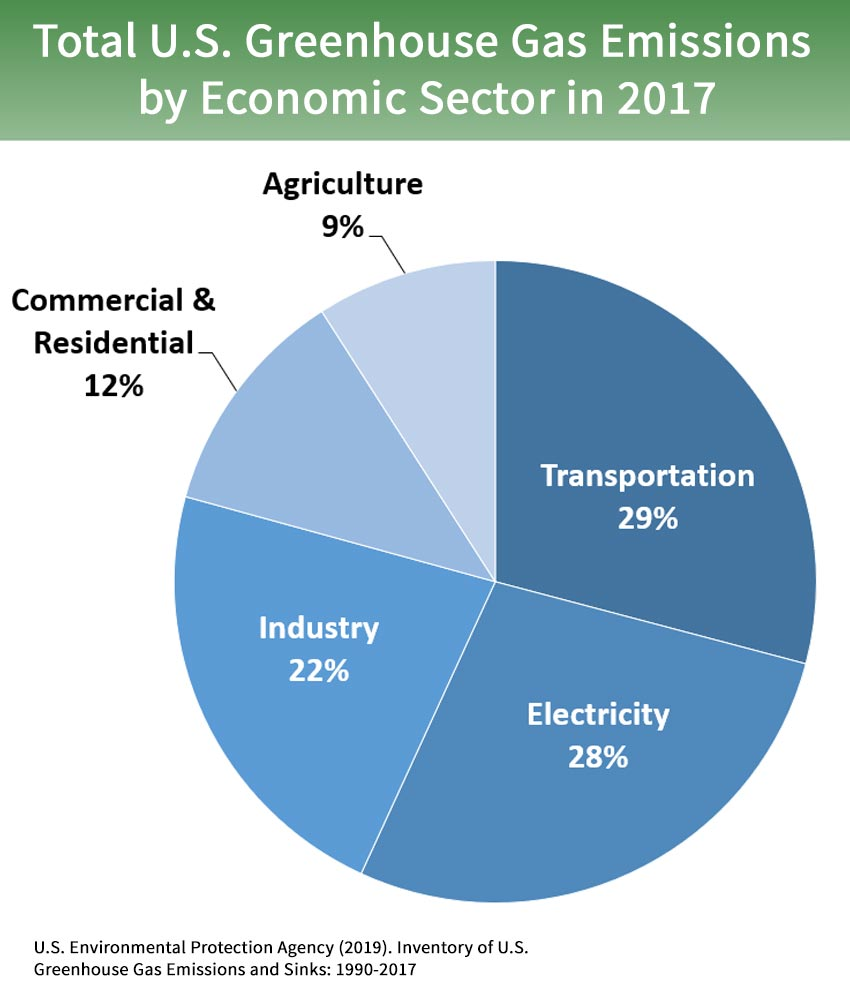
\includegraphics[width=0.6\linewidth]{figures/total-ghg-2019-caption.jpg}
	\hfill
	\caption{Total U.S. GHG Emissions by Economic Sector in 2017 \cite{us_epa_sources_2020}.}
	\label{fig:ghg}
\end{figure}

One possible solution to reduce carbon emissions, and even achieve a net zero carbon production, is to develop a hydrogen economy as the state of California is currently doing \cite{brown_economic_2013}. Some hydrogen production methods reduce, but do not eliminate, the production of CO$_2$. Nuclear reactors introduce a solution to this problem by providing clean energy to produce H$_2$.

Micro-reactors are an innovative technology that is attractive for hydrogen production. This type of reactor has three main features: factory fabricated, transportable, and self-regulating. All of the components are fully assembled in a factory and shipped out to location, reducing capital costs and enabling rapid deployment. Simple design concepts eliminate the need for a large number of specialized operators. Moreover, they utilize passive safety systems that prevent overheating or meltdown \cite{noauthor_ultimate_2019}.

The purpose of this abstract is to review and evaluate methods of hydrogen production for a hydrogen economy at the UIUC campus.
Section \ref{section:hydroprod} presents several methods and Section \ref{method} explains the methodology to calculate the amount of hydrogen required to fuel Champaign-Urbana Mass Transit District (MTD) bus system and UIUC campus fleet service vehicles, as well as the amount of CO$_2$ produced by both fleets.

\section{Hydrogen Production Methods}
\label{section:hydroprod}

Some hydrogen production processes are: 
\begin{description}[font=$\bullet$\scshape\bfseries]
	\item[] Steam-Methane Reforming (aka Natural Gas Reforming).
	\item[] Electrolysis.
	\item[] High-Temperature Electrolysis.
	\item[] Iodine-Sulfur Thermochemical Cycle.
	\item[] Coal Gasification with CCS (aka Carbon Sequestration).
	\item[] Solar Thermochemical Hydrogen Production.
\end{description}

The following subsections describe some of these methods.

\subsection{Steam Reforming}

Steam reforming is currently the least expensive way to produce hydrogen. This method separates hydrogen atoms from carbon atoms in methane (CH$_4$). This process results in carbon dioxide emissions.
Steam reforming is a mature production process that uses high-temperature steam (700$^{\circ}$C-1000$^{\circ}$C) to produce hydrogen from a methane source. Methane reacts with steam under 3-25 bar pressure in the presence of a catalyst to produce hydrogen, carbon monoxide, and a small portion of carbon dioxide. The reaction is endothermic and requires the supply of heat to occur \cite{noauthor_hydrogen_nodate}:

\begin{align}
CH_4 + H_2O + heat & \rightarrow CO + 3H_2
\label{eq:1}
\end{align}

A secondary reaction known as water-gas shift reaction occurs producing CO$_2$ and more hydrogen:
\begin{align}
CO + H_2O & \rightarrow CO_2 + H_2
\label{eq:2}
\end{align}

Although the method produces CO$_2$, vehicles reduce their GHG emissions in half \cite{noauthor_hydrogen_nodate}.

\subsection{Electrolysis}

Electrolysis is the process of using an electric current to split water into hydrogen and oxygen, Figure \ref{fig:electro}. The reaction takes place in a unit called electrolyzer. Electrolyzers consist of an anode and a cathode separated by an electrolyte. Different electrolyzers function in slightly different ways. A few types are polymer electrolyte membrane, alkaline, and solid oxide electrolyzers.

\begin{figure}[]
	\centering
	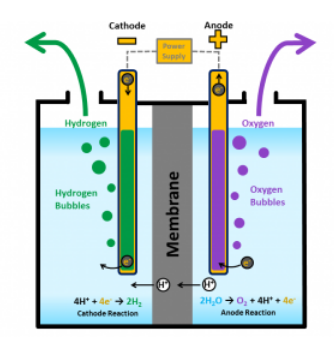
\includegraphics[width=0.55\linewidth]{figures/electrolysis.png}
	\hfill
	\caption{Production of hydrogen by electrolysis \cite{noauthor_hydrogen_nodate}.}
	\label{fig:electro}
\end{figure}

\subsection{High-Temperature Electrolysis (HTE)}

Solid oxide electrolyzers must operate at temperatures high enough for the solid oxide membranes to function properly (about 700$^{\circ}$-800$^{\circ}$C). The use of heat at these elevated temperatures decreases the amount of electrical energy needed to produce hydrogen from water. In the HTE process, thermal energy rather than electricity converts water to steam and then the electricity dissociates the water at the cathode to form hydrogen molecules \cite{xu_introduction_2017}.

\subsection{Iodine-Sulfur Thermochemical Cycle}

The concept of using nuclear heat and water allows the possibility of a sustainable production without GHG. The most efficient methods operate at considerably high temperatures, typically above 900$^{\circ}$C. For example, sulfur-based cycles (Figure \ref{fig:isulfur}) use a sulfuric acid dissociation reaction that only works above 870$^{\circ}$C and whose efficiency increases with temperature \cite{cea_gas-cooled_2006}. The sulfur-iodine (SI) cycle results the best cycle for coupling to a high temperature reactor (HTR) due to its high efficiency. A General Atomics experiment has operated multiple times to produce hydrogen. The production was at a rate of 75 L/min. The same report estimates that a scale-up of the process using a 50 MWth Nuclear Reactor could produce 12000 kg/day of hydrogen \cite{benjamin_russ_sulfur_2009}.
Another example of hydrogen production is by the Next Generation Nuclear Plant (NGNP) \cite{macdonald_ngnp_2003} which aims to produce 500 kg/h of H$_2$ by using 50 MWth \cite{cea_gas-cooled_2006}.

\begin{figure}[H]
	\centering
	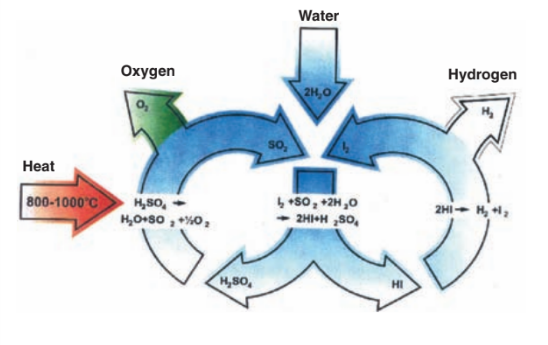
\includegraphics[width=0.85\linewidth]{figures/iodine-sulfur.png}
	\hfill
	\caption{Production of hydrogen by iodine-sulfur thermochemical cycle.}
	\label{fig:isulfur}
\end{figure}

\section{Methodology}
\label{method}

A gasoline gallon equivalent (GGE) is the amount of fuel that has the same amount of energy as a gallon of gasoline. One kilogram of hydrogen is equivalent to one gallon of gasoline \cite{noauthor_hydrogen_nodate}. Burning a gallon of gasoline produces 19.64 lbs of CO$_2$ \cite{noauthor_how_2014}. 
Similarly, a diesel gallon equivalent (DGE) has the same amount of energy as a gallon of diesel. Approximately, a DGE is 113\% of a GGE \cite{noauthor_fuel_2014}, then 1.13 Kg of hydrogen is equivalent to one gallon of diesel.
A gallon of diesel produces 22.38 lbs of CO$_2$ \cite{noauthor_how_2014}. 
Table \ref{tab:meth} summarizes this information.

\begin{table}[!h]
	\centering
    \caption{GGE, DGE, and CO$_2$ produced.}
    \label{tab:meth}
	\begin{tabular}{l|lll}
	\hline
	                 & Hydrogen & Gasoline    & Diesel      \\ \hline
	GGE              & 1 Kg     & 1 Gallon    & 0.88 Gallon \\
	DGE              & 1.13 Kg  & 1.13 Gallon & 1 Gallon    \\
    CO$_2$ produced  & -        & 19.64 lbs   & 22.38 lbs   \\ \hline

	\end{tabular}
\end{table}

\section{Results}

Figure \ref{fig:mtdfuel} shows the amount of diesel purchased every day by MTD in a year \cite{mtd_irecords_2019}. The calculations take into account the assumption that MTD consumed the purchased fuel on the same day.
Table \ref{tab:h2req} lists the required amounts of hydrogen to supply the MTD fleet. Average Gallons per day refers to the total amount of fuel consumed in a year averaged in 365 days. 

\begin{figure}[!h]
	\centering
	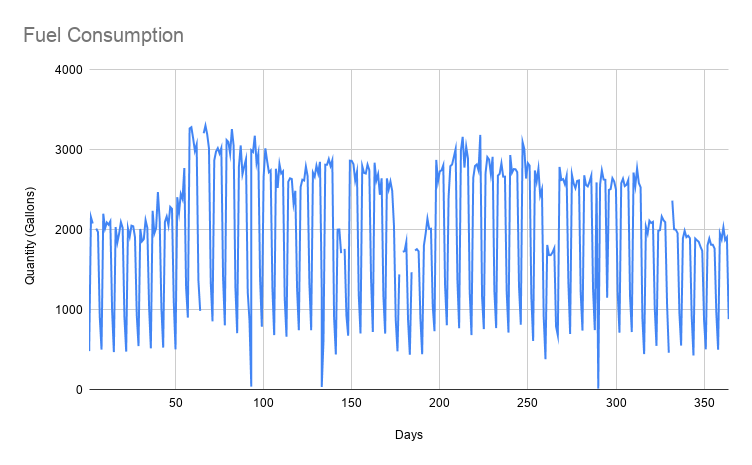
\includegraphics[width=1.05\linewidth]{figures/fuelconsumption.png}
	\hfill
	\caption{Quantity of gallons of diesel consumed each day by MTD from July 1st 2018 to June 30th 2019.}
	\label{fig:mtdfuel}
\end{figure}

The UIUC fleet counts with 227 passenger vehicles and 275 service vehicles \cite{noauthor_increase_2020}. The calculations consider only 108 vehicles chosen based on their annual mileage that combined consume 269 gasoline gallons per day \cite{holcomb_fueling_2015}. Table \ref{tab:h2req} lists the required amounts of hydrogen to supply the UIUC fleet. The table also shows the amount of CO$_2$ emitted by both fleets.

\begin{table}[]
	\centering
    \caption{Hydrogen required and CO$_2$ produced by MTD and UIUC fleets.}
    \label{tab:h2req}
\begin{tabular}{l|rr}
\hline
                          & MTD(Diesel)      & UIUC(Gasoline)   \\ \hline
Average gal/day           & 1,971.8          & 269.0            \\
Kg of H$_2$/day           & 2,228.2          & 269.0            \\
CO$_2$ emitted (lbs/day)  & 44,129.5         & 5,283.2          \\
Gal/year                  & 719,717.6        & 98,185.0         \\
Kg of H$_2$/year          & 813,280.9        & 98,185.0         \\
CO$_2$ emitted (lbs/year) & 16,107,279.9     & 1,928,353.4      \\ \hline
\end{tabular}
\end{table}

\section{Conclusion}

Transportation produces large amounts of CO$_2$ in Champaign-Urbana and the United States. This has negative effects on the environment and intensifies climate change. The University of Illinois is leading by example and actively working to reduce GHG emissions on its campus. Switching to a hydrogen economy could be the answer to reducing CO$_2$ from transportation.

Nuclear energy could contribute as well. As seen before, some methods of producing hydrogen are not entirely emissions free. A micro-reactor on campus would ease the GHG emissions by producing energy for H$_2$ production regardless of weather conditions (in contrast with renewables). Additionally, the most efficient methods run at high temperatures, another reason nuclear is appealing.

Another advantage of using micro-reactors is decentralization. Hydrogen technologies still present many challenges in transportation and storage \cite{office_of_energy_efficiency_and_renewable_energy_hydrogen_2020}\cite{office_of_energy_efficiency_and_renewable_energy_hydrogen_delivery_2020} and producing fuel locally reduces the need for both.

\section{Acknowledments}

The authors thank MTD for their contributions to the development of this document.

%%%%%%%%%%%%%%%%%%%%%%%%%%%%%%%%%%%%%%%%%%%%%%%%%%%%%%%%%%%%%%%%%%%%%%%%%%%%%%%%
\bibliographystyle{ans}
\bibliography{bibliography}
\end{document}
